%%%%%%Julia descrition starts

\section{Julia} \label{sec:julia-start}
Julia is a high-level, high-performance dynamic programming language for
technical computing, with a syntax familiar to users of other technical computing
environments \cite{julia-ref}. While it is a general-purpose language and can be used to write any
application, many of its features are well suited for numerical analysis and
computational science. Julia provides a sophisticated compiler, distributed
parallel execution, numerical accuracy, and an extensive mathematical function
library.

% This is a set of tools that provide functionality in Julia, to program the \arduino. 

\subsection{Downloading and installing on Windows} \label{julia-install-windows}
This book uses Julia 1.6.0 for demonstrating the experiments, both on Windows and Linux.
Julia does not use indentation to indicate a block of code, unlike Python. However,
the users are advised to install a programmer text editor like Atom. This editor will
allow the readers to modify the Julia source files on their machines if they want to.
Alternatively, one can also use Notepad (on Windows) or gedit (on Linux Ubuntu) to edit
Julia source files. Starting from download, we shall go through the steps to set
up Julia 1.6.0 on Windows OS:
\begin{enumerate}
      \item Visit the URL {\tt https://julialang.org/}.  At the top of the page,
            locate the Download tab and click on it. From the Current stable release,
            download the required Julia binaries (32 or 64-bit) for Windows, as shown in \figref{julia-download}.
            At the time of writing this book, the Current stable release refers to Julia 1.6.0, as shown in \figref{julia-download}. In this book, we will perform
            experiments with a 64-bit installation of Julia 1.6.0.
      \item Locate the executable file. Right-click on it and hit
            Run as administrator to begin the installation. After selecting the Installation Directory,
            a window named Select Additional Tasks appears as shown in \figref{julia-windows-install}.
            In this window, check the box which says, Add Julia to PATH and click on Next to continue the installation.
\end{enumerate}

\begin{figure}
      \centering
      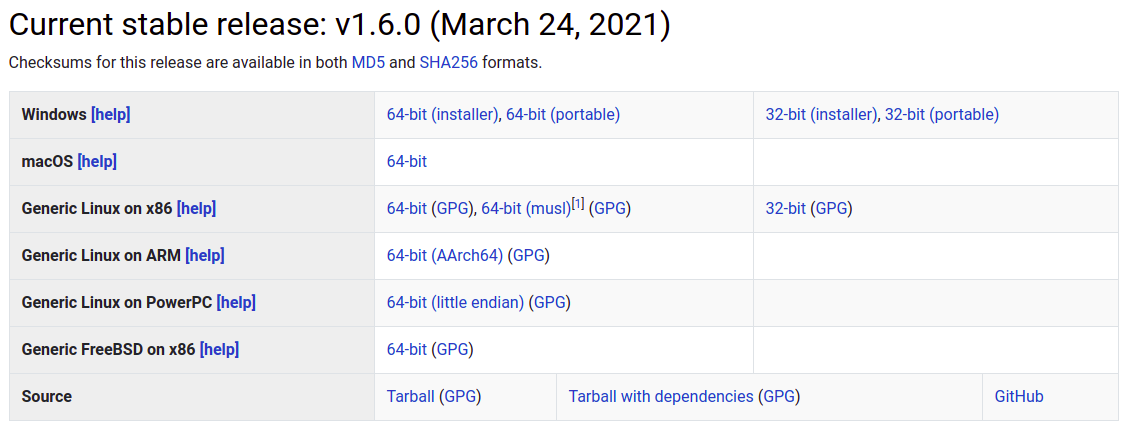
\includegraphics[width=\textwidth]{\LocSWfig/julia-download.png}
      \caption{Julia's website to download 64-bit Windows/Linux binaries}
      \label{julia-download}
\end{figure}

\begin{figure}
      \centering
      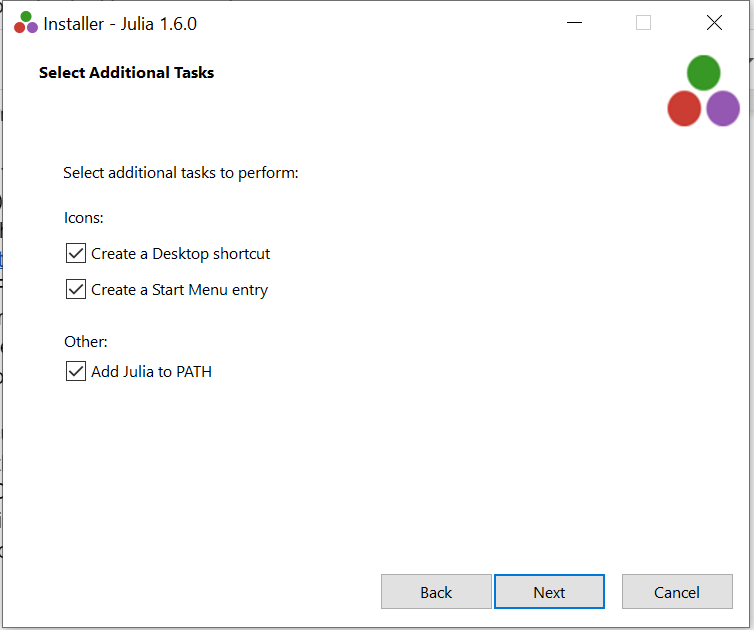
\includegraphics[width=\lgfig]{\LocSWfig/julia-windows-install.png}
      \caption{Installing Julia 1.6.0 on Windows}
      \label{julia-windows-install}
\end{figure}

\begin{figure}
      \centering
      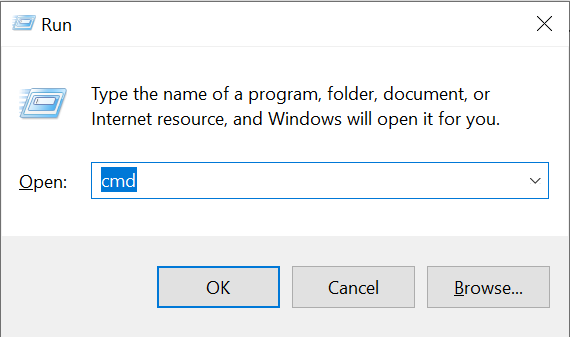
\includegraphics[width=\lgfig]{\LocSWfig/windows-cmd.png}
      \caption{Launching the Command Prompt on Windows}
      \label{windows-run-julia}
\end{figure}

\begin{figure}
      \centering
      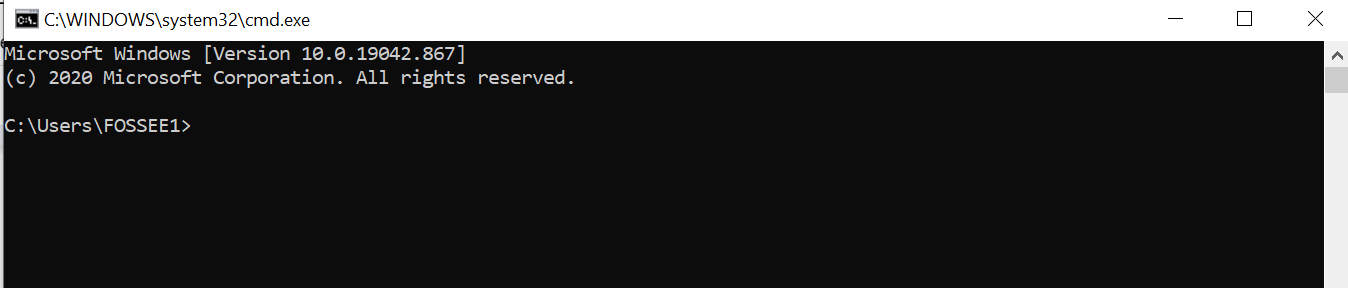
\includegraphics[width=\lgfig]{\LocSWfig/win-command-prompt.png}
      \caption{Command Prompt on Windows}
      \label{windows-cmd-julia}
\end{figure}
Once the installation is finished, Julia 1.6.0 App can be launched either
from the Start menu or from the Command Prompt. In this book, we will use the Command
Prompt to execute the Julia source files. Please note that a Julia source file has .jl as its extension.
Carry out the steps given below to execute a Julia source file from the Command Prompt:
\begin{enumerate}
      \item Launch the Command Prompt. Press the Windows key+R together. A window, as shown in \figref{windows-run-julia}
            appears. In the text box adjacent to Open, type {\tt cmd}, and press Enter. The Command Prompt, as shown in
            \figref{windows-cmd-julia} appears. By default, it points to the home directory.
      \item Now, we will check whether Julia 1.6.0 was installed successfully or not.
            In the Command Prompt, type {\tt julia -{}-version} and press Enter.
            If this step displays julia version 1.6.0 in the following line, the installation was successful.
      \item Using the {\tt cd} command, navigate to the directory where your Julia source file is located.
            Assuming that your Command Prompt points to the
            home directory, and you want to navigate to the folder Origin on
            Desktop, execute the following command: {\tt cd Desktop\textbackslash Origin} \\
            It may be noted that a backslash (\textbackslash) has been used between
            Desktop and Origin.
      \item To view the contents of this folder, type {\tt dir} and press Enter.
      \item Suppose you have a Julia source file named {\tt FILENAME.jl} in this
            folder. To execute this script, type {\tt julia FILENAME.jl} and press
            Enter. The required output will be displayed in the Command Prompt itself.
            We don't expect the readers to run the command {\tt julia FILENAME.jl} at
            this instant. This command will be helpful while running the Julia
            source files in the upcoming sections and chapters.
      \item To exit the Command Prompt, type {\tt exit} and press Enter.
\end{enumerate}

Apart from Julia, we need to install the SerialPorts \cite{julia-serial-ports} package in Julia. This package will be
required to establish serial communication with Arduino boards. Please make sure that
you are connected to the Internet. To install the package, we will use {\tt Pkg}.
It is Julia's built-in package manager and handles operations such as installing,
updating and removing packages in Julia. To install the SerialPorts package, carry out the steps given below:
\begin{enumerate}
      \item Launch the Command Prompt, as shown in \figref{windows-run-julia}.
      \item In the Command Prompt, type {\tt julia} and press Enter. It should launch Julia in an interactive session (also known as a read-eval-print loop or "REPL"), as shown
            in \figref{julia-repl-windows}. When run in interactive mode, Julia displays a banner and
            prompts the user for input. By default, Julia REPL appears in Julian prompt. It is the default mode of
            operation; each new line initially starts with {\tt julia>}, as
            shown in \figref{julia-repl-windows}. It is here that you can enter Julia expressions.
            Hitting return or Enter after a complete expression has been entered will evaluate
            the entry and show the result of the last expression.
            \begin{figure}
                  \centering
                  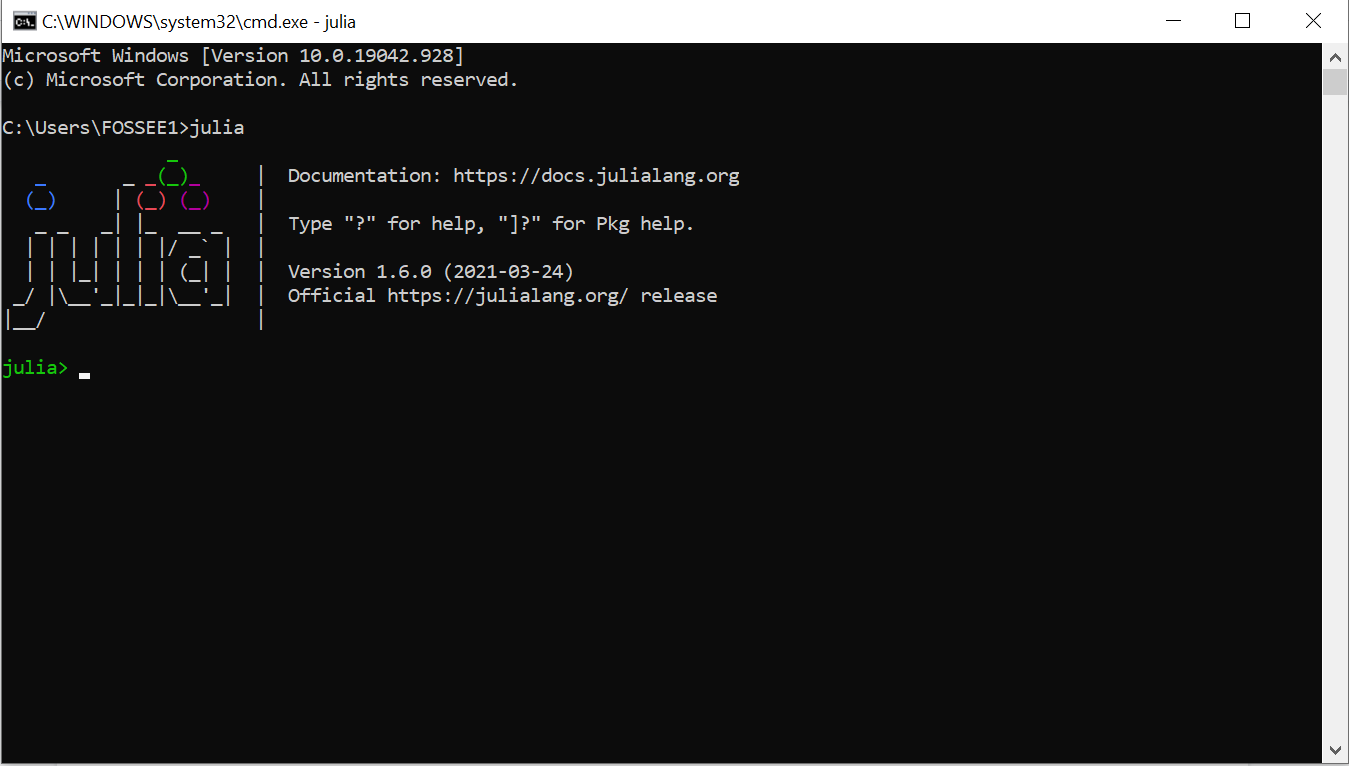
\includegraphics[width=\textwidth]{\LocSWfig/julia-repl-windows.png}
                  \caption{Windows command prompt to launch Julia REPL}
                  \label{julia-repl-windows}
            \end{figure}
      \item Now, we need to enter the {\tt Pkg} REPL in Julia. From the Julia REPL,
            press {\tt ]} to enter the {\tt Pkg} REPL. The moment you press
                  {\tt ]}, you enter {\tt Pkg} REPL, as shown in \figref{julia-pkg-windows}.
            \begin{figure}
                  \centering
                  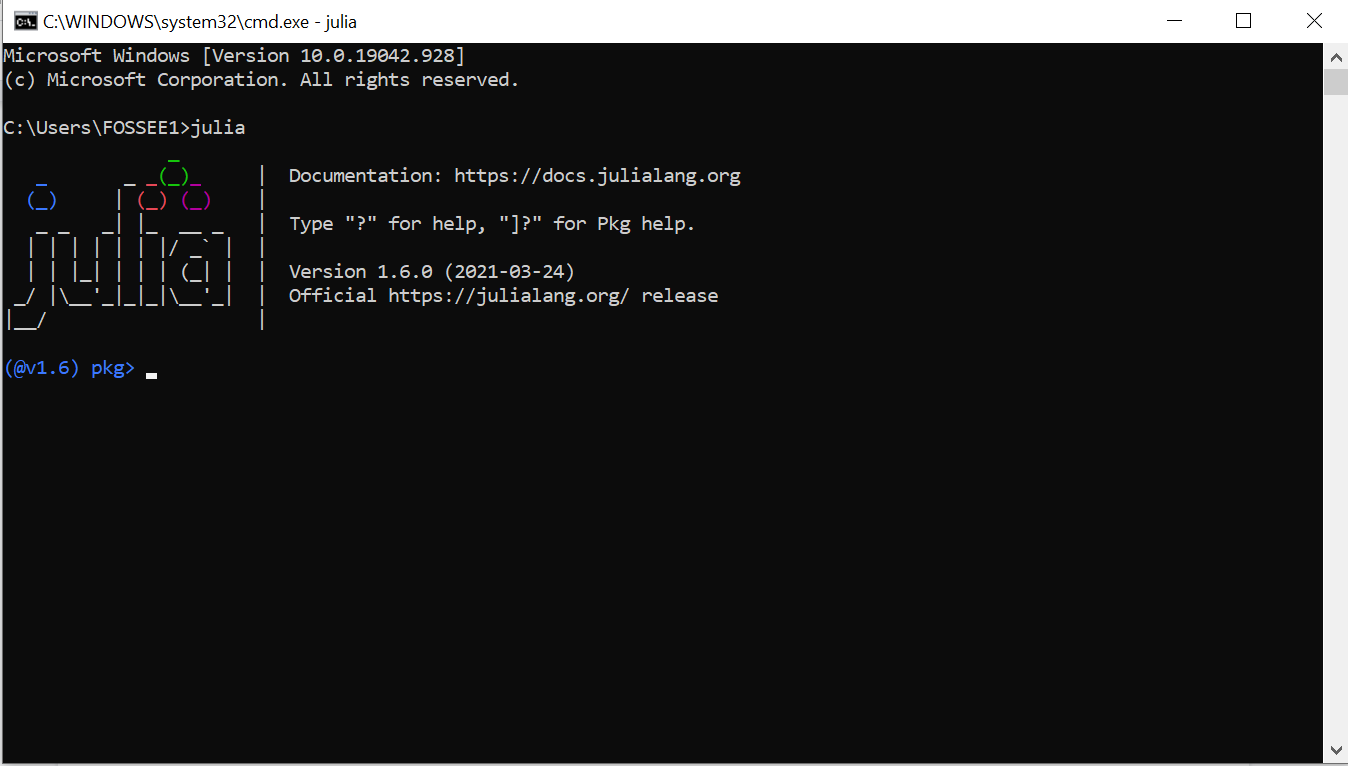
\includegraphics[width=\textwidth]{\LocSWfig/julia-pkg-windows.png}
                  \caption{Windows command prompt to enter Pkg REPL in Julia}
                  \label{julia-pkg-windows}
            \end{figure}
      \item In {\tt Pkg} REPL, type {\tt add SerialPorts} and press Enter. It might take a few seconds/minutes
            to get this package installed. Once it is installed, {\tt Pkg} REPL should show a message,
            like "3 dependencies successfully precompiled in 9 seconds (4 already precompiled)."
\end{enumerate}

We can also check the status of this package to verify whether it has been installed
successfully or not. For this, we need to get back to Julia REPL. Inside {\tt Pkg}
REPL, press backspace. The moment you press backspace, you get back to Julia REPL, as shown in
\figref{julia-repl-windows}. Now, type {\tt using Pkg} and press Enter. This command will not
generate any output. Now type {\tt Pkg.status()} and press Enter. It should display the
list of packages installed in Julia's environment. Please make sure that SerialPorts
is present in the list of packages being shown. To exit the interactive session, type CTRL+D or type {\tt exit()}.

\subsection{Downloading and installing GNU/Linux Ubuntu} \label{julia-install-linux}
We will now explain the installation of Julia on the GNU/Linux operating system.
We shall perform the installation on the 64-bit Ubuntu 18.04 LTS operating system.
These instructions will work for other GNU distributions, too, with little or
no modification. This book uses Julia 1.6.0. To install it, carry out the steps
given below:
\begin{enumerate}
      \item First, update your system. Open the Terminal. Type
                  {\tt sudo apt-get update} and press Enter.
      \item Find out your operating system support for 64-bit
            instructions. Open the Terminal. Type {\tt uname -m} and press Enter. If it returns ``x86\_64'', then your computer has 64-bit
            operating system.
      \item Visit the URL {\tt https://julialang.org/}.  At the top of the page,
            locate the Download tab and click on it. From the Current stable release, download the
            required Linux binaries (32 or 64-bit) for Generic Linux on x86, as shown in \figref{julia-download}.
            At the time of writing this book, the Current stable release refers to Julia 1.6.0,
            as shown in  \figref{julia-download}. In this book, we will perform experiments with a 64-bit installation of Julia  v1.6.0.
      \item Locate the executable (tar.gz) file. Assuming that you have downloaded the tar file in {\tt Downloads} directory, perform the following
            steps on the Terminal:
            \begin{quote}
                  {\tt cd {\large\textasciitilde}/Downloads\\
                        tar -xvzf julia-1.6.0-linux-x86\_64.tar.gz\\
                        sudo cp -r julia-1.6.0 /opt/}
            \end{quote}
      \item Finally, create a symbolic link to {\tt julia} inside the
                  {\tt /usr/local/bin} folder. In the same Terminal session from the previous step, issue the
            following command: \\
            {\tt sudo ln -s /opt/julia-1.6.0/bin/julia /usr/local/bin/julia}
\end{enumerate}

Julia is now installed and can be invoked from the Terminal. There are two modes in which Julia
source files can be executed: Interactive mode and Non-interactive mode. In this book,
we will execute source files in the latter mode i.e., from the Terminal. The readers are encouraged to explore
the former mode on their own. Please note that a Julia source file has .jl
as its extension. Carry out the steps given below to execute a Julia source file from
the Terminal:
\begin{enumerate}
      \item Open a Terminal by pressing Ctrl+Alt+T keys together.
      \item Now, we will check whether Julia 1.6.0 was installed successfully or not.
            In the Terminal, type {\tt julia -{}-version} and press Enter.
            If this step displays {\tt julia version 1.6.0} in the following line, the installation was successful.
      \item Using the {\tt cd} command, navigate to the directory where your Julia source file is located.
            Assuming that your Terminal points to the
            home directory, and you want to navigate to the folder Origin on
            Desktop, execute the following command: {\tt cd Desktop/Origin/}
      \item Suppose you have a Julia source file named {\tt FILENAME.jl} in this
            folder. To execute this script, type {\tt julia FILENAME.jl} and press
            Enter. The required output will be displayed in the Terminal itself.
            We don't expect the readers to run the command {\tt julia FILENAME.jl} at
            this instant. This command will be helpful while running the Julia
            source files in the upcoming sections and chapters.
\end{enumerate}

\begin{figure}
      \centering
      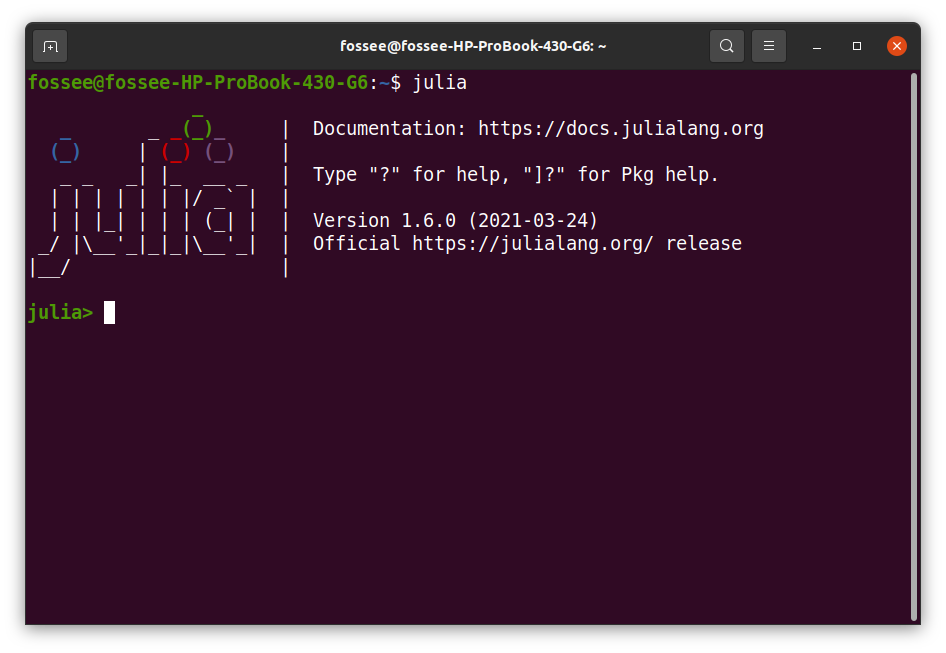
\includegraphics[width=\textwidth]{\LocSWfig/julia-terminal-repl.png}
      \caption{Linux terminal to launch Julia REPL}
      \label{julia-repl}
\end{figure}


Now, we will install a package named SerialPorts \cite{julia-serial-ports}. This package will be required to
establish serial communication with Arduino boards. Please ensure that you
are connected to the Internet. To install the package,
we will use {\tt Pkg}. It is Julia's built-in package manager and
handles operations such as installing, updating, and removing packages in Julia.
For installing LibSerialPort, carry out the steps given below:
\begin{enumerate}
      \item Open a Terminal by pressing Ctrl+Alt+T keys together. Type {\tt julia} and press Enter.
            It should launch Julia in an interactive session (also known as a read-eval-print loop or "REPL"), as shown
            in \figref{julia-repl}. When run in interactive mode, Julia displays a banner and
            prompts the user for input. By default, Julia REPL appears in Julian prompt. It is the default mode of
            operation; each new line initially starts with {\tt julia>}, as
            shown in \figref{julia-repl}. It is here that you can enter Julia expressions.
            Hitting return or Enter after a complete expression has been entered will evaluate
            the entry and show the result of the last expression.
      \item From the Julia REPL, press {\tt ]} to enter the {\tt Pkg} REPL. The moment you press
                  {\tt ]}, you enter {\tt Pkg} REPL, as shown in \figref{julia-pkg}.
      \item In {\tt Pkg} REPL, type {\tt add SerialPorts} and press Enter. It might take a few seconds
            to get this package installed. Once it is installed, {\tt Pkg} REPL should show a message,
            like "5 dependencies successfully precompiled in 12 seconds."
\end{enumerate}

\begin{figure}
      \centering
      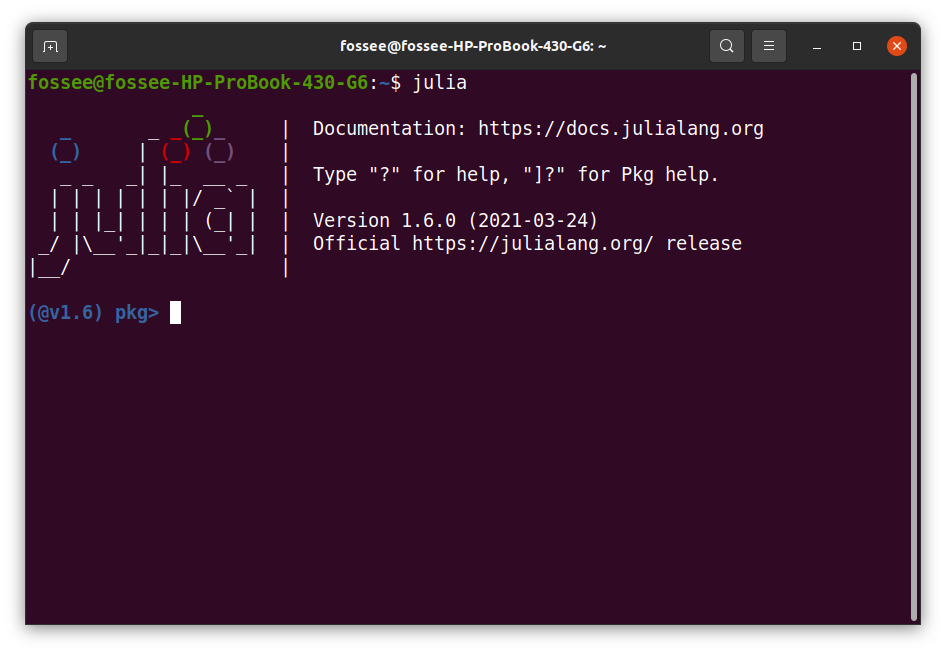
\includegraphics[width=\textwidth]{\LocSWfig/julia-pkg.png}
      \caption{Linux terminal to enter Pkg REPL in Julia}
      \label{julia-pkg}
\end{figure}

We can also check the status of this package to verify whether it has been installed
successfully or not. For this, we need to get back to Julia REPL. Inside {\tt Pkg}
REPL, press backspace. The moment you press backspace, you get back to Julia REPL, as shown in
\figref{julia-repl}. Now, type {\tt using Pkg} and press Enter. This command will not
generate any output. Now type {\tt Pkg.status()} and press Enter. It should display the
list of packages installed in Julia's environment. Please make sure that SerialPorts
is present in the list of packages being shown. To exit the interactive session, type CTRL+D or type {\tt exit()}.


\subsection{Julia-Arduino toolbox}
\label{sec:julia-toolbox}
Julia, by default, does not have the capability to connect to Arduino.
All such add-on functionalities are added to Julia using toolboxes.
Julia-Arduino toolbox can be found inside the {\tt Origin/tools/julia} directory,
see \fnrefp{fn:file-loc}.  This toolbox is compatible for both of the operating systems: Windows and Linux.
The Julia source files (or codes) for various experiments mentioned throughout this book can be found in
      {\tt Origin/user-code} directory. The {\tt user-code} directory will have many sub-directories as per the experiments.

In this book, we have created a module named "ArduinoTools" in Julia.  This module is available at
      {\tt Origin/tools/julia}. This module makes use of the functions available in the SerialPorts package to
establish serial communication with Arduino. In this module, we have added functions required to run
various experiments on \arduino. Using this basic set of functions, the user can define other functions to operate
upon the Arduino.

% Please note that the module "ArduinoTools" and the Arduino firmware  given in \ardref{ard:firmware} are required to run the experiments. 

Now, we will see how to import (or load) the module named "ArduinoTools.jl" inside a Julia source file to run
various experiments provided in this book. In a Julia source file, add {\tt include("ArduinoTools.jl")} at the top of the file.
When we add {\tt include("ArduinoTools.jl")} in a source file, the function "include" searches for "ArduinoTools.jl"
only in that directory where our source file is saved. That's why all the source files in Julia
must be saved in a folder that contains the file "ArduinoTools.jl." In this book, "ArduinoTools.jl" has been saved
in the folder where the Julia source files for each chapter are available. For the sake of convenience, we have
added {\tt include("ArduinoTools.jl")} in all the Julia source files provided in this book.
To run a particular experiment, one can follow the steps as given in \secref{julia-install-windows} and \secref{julia-install-linux}.

\subsection{Firmware}
\lstset{style=mystyle}
\label{sec:test-firmware-julia}
\addtocontents{cod}{\protect\addvspace{\codclr}}
We have provided a Julia source file (code) to check whether the firmware has been
properly installed.  That file is listed below.  Please ensure that
you have uploaded the FLOSS firmware given in \ardref{ard:firmware} on \arduino.

\begin{juliacode}
      \jcaption{A Julia source file to check whether the firmware is properly installed
            or not}{A Julia source file (code) to check whether the firmware is properly installed
            or not.  Available at
            \LocFIMjuliabrief{test\_firmware.jl}. Execute this source file by following the steps
            given in \secref{julia-install-windows} and \secref{julia-install-linux}. If the execution is
            successful, you should expect three "ok" messages. }
      \label{julia:test-firmware}
      \lstinputlisting{\LocFIMjuliacode/test_firmware.jl}
\end{juliacode}



